\documentclass[11pt,a4paper]{article}

\usepackage[T1]{fontenc}
\usepackage[utf8]{inputenc}
\usepackage{lmodern}
\usepackage[margin=2.2cm]{geometry}
\usepackage{amsmath,amssymb,amsthm,mathtools}
\usepackage{bm}
\usepackage{booktabs}
\usepackage{array}
\usepackage{xcolor}
\usepackage{tikz}
\usepackage{pgfplots}
\pgfplotsset{compat=1.18}
\usetikzlibrary{arrows.meta,calc,positioning,patterns,decorations.pathmorphing,decorations.pathreplacing,fit,backgrounds}
\usepackage{enumitem}
\usepackage[colorlinks=true,linkcolor=blue!60!black,citecolor=blue!60!black,urlcolor=blue!60!black]{hyperref}

\setlength{\emergencystretch}{3em}
\setlength{\parskip}{1.8pt}
\newcolumntype{L}[1]{>{\raggedright\arraybackslash}p{#1}}

\definecolor{atomblue}{RGB}{41,128,185}
\definecolor{defectred}{RGB}{211,47,47}
\definecolor{okgreen}{RGB}{46,125,50}
\definecolor{amberh}{RGB}{230,135,15}
\definecolor{slateh}{RGB}{82,96,109}
\definecolor{boxbg}{RGB}{245,248,252}
\definecolor{boxframe}{RGB}{180,200,225}
\definecolor{warnbg}{RGB}{255,248,235}
\definecolor{warnframe}{RGB}{225,180,100}
\definecolor{softblue}{RGB}{220,236,248}
\definecolor{softred}{RGB}{252,226,226}
\definecolor{softamber}{RGB}{254,240,210}

\newcommand{\R}{\mathbb{R}}
\newcommand{\Z}{\mathbb{Z}}
\newcommand{\T}{^{\mathsf T}}
\newcommand{\mT}{^{-\mathsf T}}
\newcommand{\tr}{\operatorname{tr}}
\newcommand{\Cred}{\tilde{\mathbf{C}}}
\newcommand{\code}[1]{\texttt{#1}}
\newcommand{\dS}{\Delta\Sigma}
\newcommand{\dW}{\Delta W}
\newcommand{\dsigbar}{\Delta\bar{\sigma}_{xy}}
\newcommand{\sigbar}{\bar{\sigma}_{xy}}
\newcommand{\sigloc}{\sigma_{\mathrm{loc}}}
\newcommand{\dsigloc}{\Delta\sigma_{\mathrm{loc}}}
\newcommand{\dgamp}{\delta\gamma_p}
\newcommand{\mutil}{\tilde{\mu}}

\newtheorem{proposition}{Proposition}
\newtheorem{remark}{Remark}

\newenvironment{keyidea}[1][Key Physical Idea]{%
  \par\medskip\noindent
  \begin{tikzpicture}
    \node[draw=boxframe,fill=boxbg,rounded corners=4pt,inner sep=10pt,text width=\dimexpr\textwidth-22pt\relax] (box) \bgroup
    \textbf{\textcolor{blue!60!black}{#1.}}\par\smallskip
}{%
    \egroup;
  \end{tikzpicture}\par\medskip
}

\newenvironment{cautionbox}[1][Subtlety / Common Pitfall]{%
  \par\medskip\noindent
  \begin{tikzpicture}
    \node[draw=warnframe,fill=warnbg,rounded corners=4pt,inner sep=10pt,text width=\dimexpr\textwidth-22pt\relax] (box) \bgroup
    \textbf{\textcolor{orange!75!black}{#1.}}\par\smallskip
}{%
    \egroup;
  \end{tikzpicture}\par\medskip
}

\title{\textbf{Stress-Drop and Energy-Drop Scaling During Avalanches in the Mesoscopic Tensorial Model (MTM)}\\[6pt]
\large Strain Control, Orowan Kinematics, Local vs.\ Macroscopic Unloading, and Pre- vs.\ Postyield Power Laws}
\author{MTM Technical Reference Note}
\date{November 2026}

\begin{document}
\maketitle

\begin{abstract}
\noindent
During athermal quasistatic (AQS) loading in the 2D Mesoscopic Tensorial Model (MTM) --- and during fast breakaway avalanches at frozen hydrogen inventory $\theta_L$ in coupled hydrogen--plasticity simulations --- each discrete instability drops both the macroscopic shear stress ($\dsigbar$, or extensive $\dS = A\,\dsigbar$) and the total elastic energy ($\dW = W_1 - W_2$). Intuition built on a spatially uniform box predicts that small avalanches on a finite stress plateau satisfy a \emph{linear} relation $\dW \approx (\sigbar/\mu)\,\dS$ ($\gamma=1$), whereas full unloading to zero stress ($\bar{\sigma}_{xy,2}\to 0$) gives a \emph{quadratic} relation $\dW = \dS^2/(2\mu A)$ ($\gamma=2$). Yet full MTM simulations of primed pseudoamorphous crystals (\emph{Phys.\ Rev.\ Mater.}\ \textbf{10}, 103611, 2026) find the exact opposite between yield regimes: \textbf{linear} scaling ($\gamma=1$, $\epsilon \approx \tau \approx 0.91$) in the \textbf{preyield} microplastic regime and \textbf{quadratic} scaling ($\gamma=2$, $\epsilon \approx 1.02$, $\tau \approx 1.25$) on the \textbf{postyield} steady-state plateau. This note resolves that apparent paradox from first principles, lists all definitions explicitly, derives the Orowan and Eshelby unloading formulas step by step, demonstrates the exact spatial-variance cancellation on a worked numerical example, and connects event-level quadratic scaling to plateau-level energy conservation.
\end{abstract}

\tableofcontents
\bigskip

% ============================================================================
\section{Complete Dictionary of Symbols, Definitions, and 2D Units}
\label{sec:definitions}
% ============================================================================

To prevent confusion between \emph{box-averaged} (macroscopic) and \emph{local} (active-zone) quantities, Table~\ref{tab:symbols} collects every symbol used throughout this note together with its physical meaning and 2D units (where energy has dimensions of $[\text{stress}]\times[\text{area}]$ in 2D per unit out-of-plane thickness).

\begin{table}[ht!]
\centering
\caption{\textbf{Glossary of geometric, kinematic, mechanical, and statistical variables in 2D MTM.}}
\label{tab:symbols}
\footnotesize
\setlength{\tabcolsep}{4.5pt}
\begin{tabular}{@{}p{4.35cm}p{9.25cm}p{2.1cm}@{}}
\toprule
\textbf{Symbol} & \textbf{Definition} & \textbf{2D Units} \\
\midrule
$\Omega_0,\; A = L_x L_y = L^2$ & Periodic 2D crystal domain and its total area & $[\text{length}]^2$ \\
$\Omega_a \subset \Omega_0,\; A_a$ & Active plastifying zone (elements switching $\mathrm{GL}(2,\Z)$ wells) and its area & $[\text{length}]^2$ \\
$\Omega_m = \Omega_0 \setminus \Omega_a$ & Elastic matrix surrounding the active avalanche patch & $[\text{length}]^2$ \\
$b,\; h$ & Burgers vector magnitude ($b=a_0$) and finite-element regularization scale & $[\text{length}]$ \\
\midrule
$\alpha \equiv \gamma_{\mathrm{tot}} = U_x/L_y$ & Imposed affine simple-shear loading parameter, $\bar{\mathbf{F}}(\alpha)=\mathbf{I}+\alpha\,\mathbf{e}_1\otimes\mathbf{e}_2$ & dimensionless \\
$\bar{\gamma}_e,\; \bar{\gamma}_p$ & Box-averaged elastic and plastic shear strains ($\gamma_{\mathrm{tot}}=\bar{\gamma}_e+\bar{\gamma}_p$) & dimensionless \\
$\dgamp(\mathbf{x})$ & Local plastic shear slip produced inside $\Omega_a$ during one avalanche & dimensionless \\
$\Delta\bar{\gamma}_p = \frac{1}{A}\int_{\Omega_0}\dgamp\,\mathrm{d}\mathbf{x}$ & Box-averaged plastic strain increment; equals $(A_a/A)\,\dgamp$ for uniform slip & dimensionless \\
\midrule
$\mu$ & Elastic shear modulus of the crystal & $[\text{stress}]$ \\
$\mutil \in (0,\mu]$ & Effective local (Eshelby) unloading modulus of $\Omega_a$: $\dsigloc = \mutil\,\dgamp$ & $[\text{stress}]$ \\
$\bar{\sigma}_{xy} \equiv \frac{1}{A}\int_{\Omega_0}\sigma_{xy}\,\mathrm{d}\mathbf{x}$ & Box-averaged Cauchy shear stress (written as $\sigma_{xy}$ in Fig.~5a of PRM 2026) & $[\text{stress}]$ \\
$\dsigbar = \bar{\sigma}_{xy,1}-\bar{\sigma}_{xy,2}$ & Macroscopic (box-averaged) shear stress drop during an avalanche & $[\text{stress}]$ \\
$\dS \equiv A\,\dsigbar$ & \textbf{Extensive macroscopic stress drop} (Sec.~V of PRM 2026) & $[\text{stress}]\cdot[\text{area}]$ \\
$\delta\sigma_{xy}(\mathbf{x}) \equiv \sigma_{xy}(\mathbf{x})-\sigbar$ & Zero-mean spatial shear-stress fluctuation ($\int_{\Omega_0}\delta\sigma_{xy}\,\mathrm{d}\mathbf{x}=0$) & $[\text{stress}]$ \\
$\sigma_{\mathrm{loc},1},\; \sigma_{\mathrm{loc},2}$ & Local shear stress inside $\Omega_a$ immediately before ($1$) and after ($2$) avalanche & $[\text{stress}]$ \\
$\dsigloc \equiv \sigma_{\mathrm{loc},1}-\sigma_{\mathrm{loc},2}$ & Local shear stress drop inside the active patch $\Omega_a$ & $[\text{stress}]$ \\
\midrule
$W = \int_{\Omega_0} w(\mathbf{x};h)\,\mathrm{d}\mathbf{x}$ & Total stored potential energy on the triangulated mesh & $[\text{energy}]$ \\
$W_{\mathrm{macro}} = \frac{A}{2\mu}\sigbar^{\,2}$ & Stored elastic energy of the spatially averaged macroscopic shear stress & $[\text{energy}]$ \\
$E_{\mathrm{inhom}} = \int_{\Omega_0}\frac{\delta\sigma_{xy}(\mathbf{x})^2}{2\mu}\,\mathrm{d}\mathbf{x}$ & Internal self-stress / grain-boundary / dislocation variance energy & $[\text{energy}]$ \\
$\dW \equiv W_1 - W_2 > 0$ & \textbf{Dissipated avalanche energy} (drop in total potential energy at fixed $\alpha$) & $[\text{energy}]$ \\
\midrule
$\gamma$ & Scaling exponent connecting energy drop to stress drop: $\dW \sim \dS^{\,\gamma}$ & dimensionless \\
$\tau,\; D_\tau$ & Power-law exponent and fractal dimension of $\dS$: $P(\dS;L)=\dS^{-\tau}\mathcal{F}(\dS/L^{D_\tau})$ & dimensionless \\
$\epsilon,\; D_\epsilon$ & Power-law exponent and fractal dimension of $\dW$: $P(\dW;L)=\dW^{-\epsilon}\mathcal{F}(\dW/L^{D_\epsilon})$ & dimensionless \\
\bottomrule
\end{tabular}
\end{table}

% ============================================================================
\section{Strain Control, \texorpdfstring{$\Delta\bar{\gamma}_e = -\Delta\bar{\gamma}_p$}{Delta gamma\_e = -Delta gamma\_p}, and Exact 2D Orowan Scaling}
\label{sec:strain_control}
% ============================================================================

\subsection{Hard-Device Strain Control vs.\ Dead-Load Stress Control}

Consider a 2D crystal of width $L_x$ and height $L_y$ subjected to simple shear $\bar{\mathbf{F}}(\alpha) = \mathbf{I} + \alpha\,\mathbf{e}_1\otimes\mathbf{e}_2$, implemented either by clamping the top wall at horizontal offset $U_x = \alpha L_y$ relative to the bottom wall or via periodic domain replication (Sec.~III of PRM 2026). The imposed geometric strain $\alpha \equiv \gamma_{\mathrm{tot}} = U_x/L_y$ is partitioned inside the crystal into two additive contributions:
\begin{equation}
\label{eq:strain_split}
\gamma_{\mathrm{tot}} = \bar{\gamma}_e + \bar{\gamma}_p,
\end{equation}
where $\bar{\gamma}_e = \sigbar/\mu$ is the reversible \emph{elastic} bond tilting (the only component that generates Cauchy shear stress) and $\bar{\gamma}_p$ is the irreversible \emph{plastic} lattice slip produced by dislocations gliding across slip planes.

During a single AQS relaxation step (\code{L-BFGS} + Delaunay edge flips at frozen $\alpha$, or at frozen $\theta_L$ in hydrogen-coupled MTM), the external grips do not move ($\Delta\gamma_{\mathrm{tot}} = 0$), so external forces perform zero work ($W_{\mathrm{ext}} = 0$). Differentiating \eqref{eq:strain_split} at fixed $\gamma_{\mathrm{tot}}$ yields:
\begin{equation}
\label{eq:hard_device}
\Delta\gamma_{\mathrm{tot}} = \Delta\bar{\gamma}_e + \Delta\bar{\gamma}_p = 0
\qquad\Longrightarrow\qquad
\Delta\bar{\gamma}_e = -\Delta\bar{\gamma}_p < 0,
\qquad
\dsigbar = -\mu\,\Delta\bar{\gamma}_e = \mu\,\Delta\bar{\gamma}_p > 0.
\end{equation}
Physically, a $+b$ slip step across an internal plane absorbs part of the fixed boundary offset $U_x$ in a new stress-free periodic minimum, allowing all surrounding elastic layers above and below the slip plane to spring back by $-\Delta\bar{\gamma}_p$ (Figure~\ref{fig:strain_control}a--b).

\begin{cautionbox}[Contrast: Hard Device (Strain Control) vs.\ Soft Device (Stress Control)]
Under \textbf{dead-load stress control} ($\sigbar = \text{const}$ instead of fixed $U_x$), we have $\Delta\bar{\gamma}_e = 0$ and $\Delta\gamma_{\mathrm{tot}} = +\Delta\bar{\gamma}_p$: the top wall displaces freely as the dislocation glides, the macroscopic stress \emph{never} drops, and a runaway avalanche does not self-arrest unless it meets an obstacle. Under \textbf{strain control} ($\gamma_{\mathrm{tot}} = \text{const}$), each increment of slip unloads the crystal ($\Delta\bar{\gamma}_e = -\Delta\bar{\gamma}_p$), producing vertical drops $\dsigbar$ at fixed $\alpha$ that self-arrest when the driving stress falls back to a threshold (Figure~\ref{fig:strain_control}c).
\end{cautionbox}

\subsection{How MTM Realizes \texorpdfstring{$\Delta\bar{\gamma}_e = -\Delta\bar{\gamma}_p$}{Delta gamma\_e = -Delta gamma\_p} Without Storing \texorpdfstring{$\gamma_e$}{gamma\_e} or \texorpdfstring{$\gamma_p$}{gamma\_p}}

Unlike phenomenological crystal plasticity, MTM does not evolve a separate plastic strain variable $\gamma_p$. Instead, the $\mathrm{GL}(2,\Z)$-invariant energy $\varphi(\mathbf{C}) = \varphi_{\mathcal{D}}(\tilde{\mathbf{C}})$ with $\tilde{\mathbf{C}} = \mathbf{m}\T\mathbf{C}\mathbf{m} \in \mathcal{D}$ encodes plastic slip directly in the integer reduction matrix $\mathbf{m} \in \mathrm{GL}(2,\Z)$ and Delaunay topology:
\begin{enumerate}[nosep]
  \item As $\alpha$ increases, triangles along an active slip plane shear out of the reference fundamental domain $\mathcal{D}$.
  \item Lagrange reduction applies the integer shear generator $\mathbf{m}_3 = \begin{pmatrix} 1 & -1 \\ 0 & 1 \end{pmatrix}$ (Eq.~10 of PRM 2026) and CGAL Delaunay edge flips reconnect vertices across the shifted lattice plane, resetting the slipped elements into an adjacent equivalent stress-free square well ($\det\tilde{\mathbf{C}}=1$). That discrete lattice shift \emph{is} $\Delta\bar{\gamma}_p$.
  \item Because outer nodes remain pinned at $U_x = \alpha L_y$ (or periodic vectors $\mathbf{R}_{(\mathbf{n})} = \bar{\mathbf{F}}(\alpha)\mathbf{t}_{(\mathbf{n})}$ stay fixed), \code{L-BFGS} equilibrates all remaining bulk triangles to smaller $\tilde{\mathbf{C}}$, automatically yielding $\Delta\bar{\gamma}_e = -\Delta\bar{\gamma}_p$ and $\dsigbar = \mu\,\Delta\bar{\gamma}_p$.
\end{enumerate}

\begin{figure}[ht!]
\centering
\resizebox{\textwidth}{!}{%
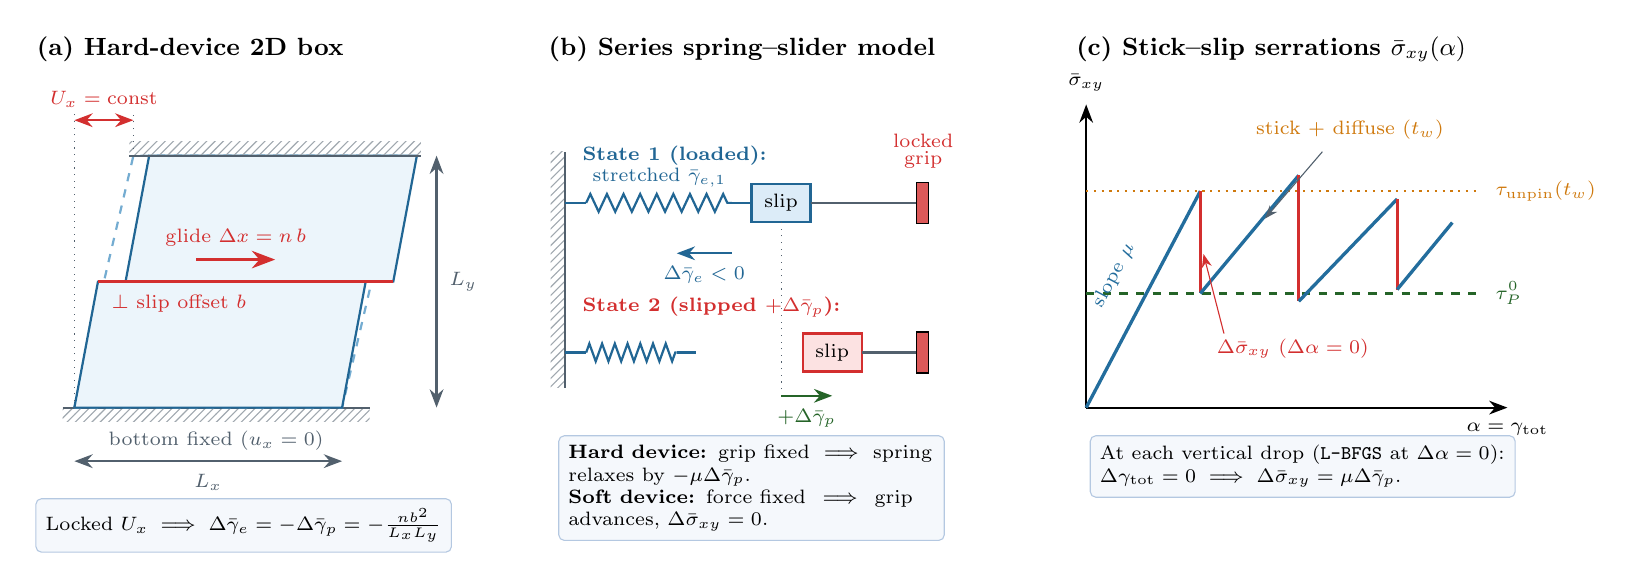
\begin{tikzpicture}[>=Stealth, font=\small]
  % ==================== PANEL (a): Strain-controlled 2D box (x = 0..5.7) ====================
  \node[anchor=west, font=\bfseries\small] at (0.0, 5.45) {(a) Hard-device 2D box};

  % Fixed bottom clamp
  \fill[pattern=north east lines, pattern color=slateh!55] (0.45, 0.72) rectangle (4.35, 0.90);
  \draw[thick, slateh] (0.45, 0.90) -- (4.35, 0.90);
  \node[font=\scriptsize, slateh] at (2.40, 0.48) {bottom fixed ($u_x=0$)};

  % Deformed box outline (tilted before -> upright after inside)
  \draw[dashed, atomblue!65, line width=0.8pt] (0.60,0.90) -- (1.35,4.10) -- (4.75,4.10) -- (4.00,0.90) -- cycle;
  % Slipped two halves (reduced bulk tilt!)
  \fill[softblue!55] (0.60,0.90) -- (0.90,2.50) -- (4.30,2.50) -- (4.00,0.90) -- cycle;
  \fill[softblue!55] (1.25,2.50) -- (1.55,4.10) -- (4.95,4.10) -- (4.65,2.50) -- cycle;
  \draw[thick, atomblue!80!black] (0.60,0.90) -- (0.90,2.50) -- (4.30,2.50) -- (4.00,0.90) -- cycle;
  \draw[thick, atomblue!80!black] (1.25,2.50) -- (1.55,4.10) -- (4.95,4.10) -- (4.65,2.50) -- cycle;

  % Top clamped grip at fixed Ux
  \fill[pattern=north east lines, pattern color=slateh!55] (1.30, 4.10) rectangle (5.00, 4.28);
  \draw[thick, slateh] (1.30, 4.10) -- (5.00, 4.10);
  \draw[<->, thick, defectred] (0.60, 4.55) -- (1.35, 4.55) node[midway, above=1pt, font=\scriptsize, text=defectred] {$U_x = \mathrm{const}$};
  \draw[dotted, slateh] (0.60, 0.90) -- (0.60, 4.68);
  \draw[dotted, slateh] (1.35, 4.10) -- (1.35, 4.68);

  % Slip plane and step +b
  \draw[very thick, defectred] (0.90, 2.50) -- (4.65, 2.50);
  \draw[->, very thick, defectred] (2.15, 2.78) -- (3.15, 2.78) node[midway, above=1pt, font=\scriptsize, text=defectred] {glide $\Delta x = n\,b$};
  \node[font=\scriptsize, text=defectred, anchor=west] at (0.95, 2.22) {$\perp$ slip offset $b$};
  \draw[<->, thick, slateh] (5.20, 0.90) -- (5.20, 4.10) node[midway, right=1pt, font=\scriptsize, text=slateh] {$L_y$};
  \draw[<->, thick, slateh] (0.60, 0.22) -- (4.00, 0.22) node[midway, below=1pt, font=\scriptsize, text=slateh] {$L_x$};

  % Equation inside panel a
  \node[draw=boxframe, fill=boxbg, rounded corners=2pt, inner sep=3.5pt, font=\scriptsize, anchor=north] at (2.75, -0.25)
    {Locked $U_x \implies \Delta\bar{\gamma}_e = -\Delta\bar{\gamma}_p = -\frac{n b^2}{L_x L_y}$};

  % ==================== PANEL (b): Spring-slider analogy (x = 6.5..12.5) ====================
  \node[anchor=west, font=\bfseries\small] at (6.50, 5.45) {(b) Series spring--slider model};

  % Frame
  \fill[pattern=north east lines, pattern color=slateh!55] (6.65, 1.15) rectangle (6.83, 4.15);
  \draw[thick, slateh] (6.83, 1.15) -- (6.83, 4.15);

  % State 1 (Before slip): center y = 3.50
  \node[font=\scriptsize\bfseries, text=atomblue!80!black, anchor=west] at (6.93, 4.10) {State 1 (loaded):};
  \draw[thick, atomblue!80!black] (6.83, 3.50) -- (7.10, 3.50);
  \draw[thick, atomblue!80!black, decorate, decoration={zigzag, segment length=6pt, amplitude=3.2pt}] (7.10, 3.50) -- (8.95, 3.50);
  \draw[thick, atomblue!80!black] (8.95, 3.50) -- (9.20, 3.50);
  \filldraw[fill=softblue, draw=atomblue!80!black, thick] (9.20, 3.26) rectangle (9.95, 3.74);
  \node[font=\scriptsize] at (9.575, 3.50) {slip};
  \draw[thick, slateh] (9.95, 3.50) -- (11.30, 3.50);
  \filldraw[fill=defectred!80, draw=black] (11.30, 3.24) rectangle (11.45, 3.76);
  \node[font=\scriptsize, text=atomblue!80!black] at (8.03, 3.82) {stretched $\bar{\gamma}_{e,1}$};

  % Middle arrow showing Delta gamma_e < 0 completely clear of labels
  \draw[->, thick, atomblue!80!black] (8.95, 2.86) -- (8.25, 2.86) node[midway, below=1pt, font=\scriptsize, text=atomblue!80!black] {$\Delta\bar{\gamma}_e < 0$};

  % State 2 (After slip): center y = 1.60
  \node[font=\scriptsize\bfseries, text=defectred, anchor=west] at (6.93, 2.18) {State 2 (slipped $+\Delta\bar{\gamma}_p$):};
  \draw[thick, atomblue!80!black] (6.83, 1.60) -- (7.10, 1.60);
  \draw[thick, atomblue!80!black, decorate, decoration={zigzag, segment length=4.6pt, amplitude=3.2pt}] (7.10, 1.60) -- (8.25, 1.60);
  \draw[thick, atomblue!80!black] (8.25, 1.60) -- (8.50, 1.60);
  \draw[dotted, slateh] (9.575, 1.05) -- (9.575, 3.26);
  \filldraw[fill=softred, draw=defectred, thick] (9.85, 1.36) rectangle (10.60, 1.84);
  \node[font=\scriptsize] at (10.225, 1.60) {slip};
  \draw[thick, slateh] (10.60, 1.60) -- (11.30, 1.60);
  \filldraw[fill=defectred!80, draw=black] (11.30, 1.34) rectangle (11.45, 1.86);
  \node[font=\scriptsize, text=defectred, align=center, anchor=south] at (11.38, 3.82) {locked\\[-2pt]grip};
  \draw[->, thick, okgreen!80!black] (9.575, 1.05) -- (10.225, 1.05) node[midway, below=1pt, font=\scriptsize, text=okgreen!80!black] {$+\Delta\bar{\gamma}_p$};

  \node[draw=boxframe, fill=boxbg, rounded corners=2pt, inner sep=3.5pt, font=\scriptsize, text width=4.65cm, anchor=north] at (9.20, 0.55)
    {\textbf{Hard device:} grip fixed $\implies$ spring relaxes by $-\mu\Delta\bar{\gamma}_p$.\\
     \textbf{Soft device:} force fixed $\implies$ grip advances, $\dsigbar=0$.};

  % ==================== PANEL (c): Stress-strain sawtooth (x = 13.3..19.7) ====================
  \node[anchor=west, font=\bfseries\small] at (13.20, 5.45) {(c) Stick--slip serrations $\sigbar(\alpha)$};

  % Axes
  \draw[->, thick] (13.45, 0.90) -- (18.80, 0.90) node[below=2pt, font=\scriptsize] {$\alpha=\gamma_{\mathrm{tot}}$};
  \draw[->, thick] (13.45, 0.90) -- (13.45, 4.75) node[above=1pt, font=\scriptsize] {$\sigbar$};

  % Bare Peierls & aged thresholds
  \draw[dashed, okgreen!80!black, thick] (13.45, 2.35) -- (18.45, 2.35) node[right=2pt, font=\scriptsize, text=okgreen!80!black] {$\tau_P^0$};
  \draw[dotted, amberh!90!black, thick] (13.45, 3.65) -- (18.45, 3.65) node[right=2pt, font=\scriptsize, text=amberh!90!black] {$\tau_{\mathrm{unpin}}(t_w)$};

  % Sawtooth curve: elastic ramp -> vertical avalanche drop
  \draw[very thick, atomblue!85!black] (13.45, 0.90) -- (14.90, 3.65);
  \draw[very thick, defectred] (14.90, 3.65) -- (14.90, 2.35);
  \draw[very thick, atomblue!85!black] (14.90, 2.35) -- (16.15, 3.85);
  \draw[very thick, defectred] (16.15, 3.85) -- (16.15, 2.25);
  \draw[very thick, atomblue!85!black] (16.15, 2.25) -- (17.40, 3.55);
  \draw[very thick, defectred] (17.40, 3.55) -- (17.40, 2.40);
  \draw[very thick, atomblue!85!black] (17.40, 2.40) -- (18.10, 3.25);

  % Annotations placed cleanly in open space
  \node[font=\scriptsize, rotate=62, inner sep=1pt, text=atomblue!85!black] at (13.80, 2.58) {slope $\mu$};
  \node[fill=white, fill opacity=0.92, text opacity=1, inner sep=1.5pt, font=\scriptsize, text=defectred, anchor=west] (dropnote) at (15.05, 1.65) {$\dsigbar$ ($\Delta\alpha=0$)};
  \draw[->, thin, defectred] (15.20, 1.84) -- (14.94, 2.85);
  \node[font=\scriptsize, text=amberh!90!black, anchor=south] at (16.80, 4.18) {stick + diffuse ($t_w$)};
  \draw[->, thin, slateh] (16.45, 4.15) -- (15.72, 3.30);

  \node[draw=boxframe, fill=boxbg, rounded corners=2pt, inner sep=3.5pt, font=\scriptsize, text width=5.15cm, anchor=north] at (16.20, 0.55)
    {At each vertical drop (\code{L-BFGS} at $\Delta\alpha=0$):\\
     $\Delta\gamma_{\mathrm{tot}}=0 \implies \dsigbar = \mu\Delta\bar{\gamma}_p$.};
\end{tikzpicture}%
}
\caption{\textbf{Origin of $\Delta\bar{\gamma}_e = -\Delta\bar{\gamma}_p$ and stress drops under strain control.} \textbf{(a)}~During an avalanche, the top wall stays fixed at $U_x$, so a lattice slip $+b$ over distance $\Delta x = n b$ reduces the elastic tilt of the remaining crystal rows. \textbf{(b)}~Equivalent 1D spring--slider at locked grip vs.\ dead load. \textbf{(c)}~Alternating quasistatic loading and hydrogen diffusion produces vertical stress drops $\dsigbar$ at fixed $\alpha$.}
\label{fig:strain_control}
\end{figure}

\subsection{Exact 2D Orowan Stress-Drop Scaling (\texorpdfstring{$b/L$}{b/L} vs.\ \texorpdfstring{$b^2/L^2$}{b\textasciicircum 2/L\textasciicircum 2})}

Care is needed not to confuse \emph{$n$ lattice hops of one dislocation} with \emph{$n$ full-width sweeps across the box}:
\begin{itemize}[nosep]
  \item \textbf{Single full-width sweep ($\Delta x = L_x$):} When one edge dislocation of Burgers vector $b$ traverses the entire box width $L_x$, the upper crystal half shifts permanently by $b$ relative to the lower half, giving
  \begin{equation}
  \Delta\bar{\gamma}_p^{\mathrm{sweep}} = \frac{b}{L_y},
  \qquad
  \dsigbar^{\mathrm{sweep}} = \mu\,\frac{b}{L_y},
  \qquad
  \dS^{\mathrm{sweep}} = \mu\,b\,L_x.
  \end{equation}
  \item \textbf{Partial $n$-hop glide ($\Delta x = n\,b < L_x$):} Moving a single dislocation only $n$ lattice spacings sweeps the fraction $\Delta x / L_x$ of the slip plane (equivalently $\Delta\bar{\gamma}_p = \rho_m b\,\Delta x$ with $\rho_m = 1/(L_x L_y)$):
  \begin{equation}
  \label{eq:orowan_nhop}
  \Delta\bar{\gamma}_p = \frac{b}{L_y}\cdot\frac{n\,b}{L_x} = \frac{n\,b^2}{A},
  \qquad
  \dsigbar = \mu\,\frac{n\,b^2}{A} \sim \mu\,n\left(\frac{b}{L}\right)^{\!2},
  \qquad
  \dS = A\,\dsigbar = \mu\,n\,b^2.
  \end{equation}
  Notice that $\dS = \mu\,n\,b^2$ is \emph{independent} of box size $A$ and proportional to the swept area $b\,\Delta x = n\,b^2$! One only obtains $\dsigbar = \mu\,N_{\mathrm{dis}} b / L_y$ when $N_{\mathrm{dis}}$ dislocations each sweep the \emph{entire} box width $L_x$.
  \item \textbf{Clamped-cylinder image back-stress (hydrogen Task~4B geometry):} In a cylinder of radius $R$ whose boundary nodes at $r=R$ are clamped to the centered Volterra field, shifting the dislocation off-center by $\Delta x = n\,b$ creates a same-sign image dislocation at $x_{\mathrm{img}} = R^2/\Delta x$, generating a restoring shear stress:
  \begin{equation}
  \Delta\tau_{\mathrm{back}}(\Delta x) \approx \frac{\mu\,b}{\pi(1-\nu_{2\mathrm{D}})}\,\frac{1}{R^2/\Delta x}
  = \frac{\mu}{\pi(1-\nu_{2\mathrm{D}})}\,\frac{n\,b^2}{R^2}.
  \end{equation}
  This exhibits the same $n(b/R)^2$ scaling as~\eqref{eq:orowan_nhop}. For the \code{LJ\_V3} hydrogen-ageing benchmark ($\mu = C_{66} = 12.404$, $\nu_{2\mathrm{D}} = 1/3$, $R = 13.5\,b$), a single $1\,b$ hop creates an image back-stress $\delta\tau_{1b} \approx 12.404 / \big[\pi(2/3)(13.5)^2\big] \approx 0.0325$, which exceeds even the $t_w\to\infty$ ageing overshoot $\Delta\tau_{\mathrm{sat}} = 0.0228$, explaining why the test dislocation self-arrests after $1.00\,a_0$. In large samples ($L$ or $R \gtrsim 30\,b$), $\delta\tau_{1b} \ll \Delta\tau_{\mathrm{age}}(t_w)$ drives multi-hop Portevin--Le~Chatelier avalanches of size $n_{\mathrm{jump}} \sim (\Delta\tau_{\mathrm{age}}/\mu)(L/b)^2$ per \code{L-BFGS} step.
\end{itemize}

% ============================================================================
\section{The Apparent Paradox: Homogeneous Unloading vs.\ MTM Power-Law Statistics}
\label{sec:paradox}
% ============================================================================

\subsection{What a Spatially Homogeneous Crystal Predicts}

Suppose first that the entire box $\Omega_0$ has spatially \emph{uniform} shear stress dropping from $\bar{\sigma}_{xy,1}$ to $\bar{\sigma}_{xy,2} = \bar{\sigma}_{xy,1} - \dsigbar$ ($\dsigbar = \dS/A$) with zero boundary work ($W_{\mathrm{ext}}=0$). Subtracting the macroscopic shear energies $W_{\mathrm{macro}} = \frac{A}{2\mu}\sigbar^{\,2}$ before and after the avalanche gives:
\begin{equation}
\label{eq:naive_homog}
\Delta W_{\mathrm{macro}} = \frac{A}{2\mu}\left(\bar{\sigma}_{xy,1}^{\,2} - \bar{\sigma}_{xy,2}^{\,2}\right)
= \frac{A}{\mu}\,\bar{\sigma}_{\mathrm{avg}}\,\dsigbar
= \frac{1}{\mu}\left(\bar{\sigma}_{xy,1}\,\dS - \frac{1}{2A}\,\dS^{\,2}\right),
\end{equation}
where $\bar{\sigma}_{\mathrm{avg}} \equiv \frac{1}{2}(\bar{\sigma}_{xy,1}+\bar{\sigma}_{xy,2})$ is the mean box stress during unloading.
Formula~\eqref{eq:naive_homog} has two limiting behaviors:
\begin{enumerate}[nosep]
  \item \textbf{Full unloading ($\bar{\sigma}_{xy,2} \to 0$, $\dS = A\,\bar{\sigma}_{xy,1}$):} The avalanche wipes out $100\%$ of the crystal's elastic strain ($\Delta\bar{\gamma}_p = \bar{\sigma}_{xy,1}/\mu$, requiring $N_{\mathrm{sweeps}} = (\bar{\sigma}_{xy,1}/\mu)(L_y/b)$ full-width sweeps in one \code{L-BFGS} call). This occurs at the \textbf{pristine-crystal spinodal yield drop} ($\alpha_c \approx 0.138$ in PRM 2026) and gives the \textbf{quadratic} ceiling:
  \begin{equation}
  \Delta W_{\mathrm{full}} = \frac{A}{2\mu}\,\bar{\sigma}_{xy,1}^{\,2} = \frac{\dS^{\,2}}{2\mu A}.
  \end{equation}
  \item \textbf{Partial unloading ($\dsigbar \ll \bar{\sigma}_{xy,1}$):} Because the background stress stays near the plateau value $\bar{\sigma}_{xy,1} > 0$, Eq.~\eqref{eq:naive_homog} keeps the first-order term and predicts \textbf{linear} scaling $\Delta W_{\mathrm{macro}} \approx (\bar{\sigma}_{xy,1}/\mu)\,\dS$ ($\gamma=1$). For a single dislocation gliding $\Delta x = n b$, Eq.~\eqref{eq:orowan_nhop} cancels $A$ cleanly to leave the Peach--Koehler work $(\bar{\sigma}_{xy,1} b)\,\Delta x$.
\end{enumerate}

\subsection{What Full MTM Actually Measures (Salman, Ahadi \& Truskinovsky, PRM 2026)}

In \emph{Phys.\ Rev.\ Mater.}\ \textbf{10}, 103611 (2026), pristine $N\times N$ square crystals ($N=100,200,400$) were first primed past their spinodal threshold $\alpha_c \approx 0.138$ to nucleate a self-equilibrated dislocation network, then loaded quasistatically in simple shear. Finite-size scaling of single-avalanche stress drops $\dS = A\,\dsigbar$ and dissipated energies $\dW$ was collapsed onto $P(s;L) = s^{-x}\mathcal{F}(s/L^{D_x})$ (Eq.~43, Fig.~10 of PRM 2026). If events satisfy a scaling relation $\dW \sim \dS^{\,\gamma}$, probability conservation $P(\dW)\,\mathrm{d}\dW = P(\dS)\,\mathrm{d}\dS$ enforces:
\begin{equation}
\label{eq:exponent_relation}
\dW^{-\epsilon}\,\dS^{\,\gamma-1} \sim \dS^{-\gamma\epsilon + \gamma - 1} \sim \dS^{-\tau}
\qquad\Longrightarrow\qquad
\epsilon - 1 = \frac{\tau - 1}{\gamma}.
\end{equation}
The measured exponents in the two regimes (Table~\ref{tab:prm_exponents}) reveal a striking reversal of the homogeneous intuition~\eqref{eq:naive_homog}:
\begin{itemize}[nosep]
  \item \textbf{Preyield (State~A, caged microplasticity):} Even though $\sigbar(\alpha)$ is rising along an elastic hardening branch, $\tau \approx \epsilon \approx 0.91$, implying \textbf{linear} event scaling $\gamma = 1$ ($\dW \sim \dS$).
  \item \textbf{Postyield (State~D, steady plateau at $\sigbar \approx 0.13$):} Even though $\sigbar$ fluctuates tightly around a nonzero steady-state plateau, $\tau = 1.2476$ and $\epsilon = 1.0207$ differ sharply; using \eqref{eq:exponent_relation} with $\gamma = 2$ predicts $\epsilon = 1 + (1.2476-1)/2 = 1.124$ (or $1.10$ for $\tau\approx 1.2$), consistent within the system-size uncertainty ($\pm 0.2$) with \textbf{quadratic} event scaling $\dW \sim \dS^{\,2}$!
\end{itemize}

\begin{table}[ht!]
\centering
\caption{\textbf{Measured MTM avalanche scaling exponents} (Salman, Ahadi \& Truskinovsky, PRM 2026, Sec.~V, Fig.~10).}
\label{tab:prm_exponents}
\footnotesize
\setlength{\tabcolsep}{4.5pt}
\begin{tabular}{@{}lcccccL{4.4cm}@{}}
\toprule
\textbf{Regime} & $\epsilon$ ($\dW$) & $D_\epsilon$ & $\tau$ ($\dS$) & $D_\tau$ & $\gamma$ ($\dW\sim\dS^{\gamma}$) & \textbf{Spatial morphology} \\
\midrule
Preyield (State A)  & $0.9195$ & $0.3640$ & $0.9070$ & $0.3987$ & $\mathbf{1}$ \textbf{(linear)}    & Isolated 0D caged clusters ($D_\epsilon \approx 0.36$) \\
Postyield (State D) & $1.0207$ & $0.9836$ & $1.2476$ & $1.4379$ & $\mathbf{2}$ \textbf{(quadratic)} & Spanning 1D branched bands ($D_\epsilon \approx 0.98$) \\
\bottomrule
\end{tabular}
\end{table}

\begin{keyidea}[The Central Question]
Why does a small avalanche on the \textbf{postyield} plateau at $\sigbar \approx 0.13 \neq 0$ obey $\dW \sim \dS^{\,2}$ instead of $\dW \approx (\sigbar/\mu)\,\dS$? And why is \textbf{preyield} linear instead?
\end{keyidea}

% ============================================================================
\section{Exact Resolution: Eshelby's Theorem and Rectangle + Triangle Decomposition}
\label{sec:eshelby}
% ============================================================================

\subsection{Exact Local Energy-Drop Formula on the MTM Mesh}

The naive formula~\eqref{eq:naive_homog} failed because it discarded internal stress heterogeneity ($\delta\sigma_{xy}(\mathbf{x}) \in [-0.5, +0.5]$ in Figs.~4--7 of PRM 2026, several times larger than the plateau average $\sigbar \approx 0.13$).

To get the \emph{exact} relation, compare two equilibrated MTM states $\mathbf{u}_1$ and $\mathbf{u}_2$ at the same boundary shear $\alpha$ ($\nabla\cdot\boldsymbol{\sigma}_1 = \nabla\cdot\boldsymbol{\sigma}_2 = \mathbf{0}$, periodic fluctuation $\Delta\mathbf{u} = \mathbf{u}_2 - \mathbf{u}_1$). Partition the total strain increment into elastic and plastic parts, $\Delta\boldsymbol{\varepsilon}(\mathbf{x}) = \Delta\boldsymbol{\varepsilon}^e(\mathbf{x}) + \Delta\boldsymbol{\varepsilon}^p(\mathbf{x})$, where $\Delta\boldsymbol{\varepsilon}^p(\mathbf{x})$ is nonzero only inside the active region $\Omega_a$. Because both $\boldsymbol{\sigma}_1$ and $\boldsymbol{\sigma}_2$ are self-equilibrated and $\Delta\mathbf{u}$ is periodic, virtual work annihilates the total strain integral:
\[
\int_{\Omega_0} \frac{\boldsymbol{\sigma}_1 + \boldsymbol{\sigma}_2}{2} : \Delta\boldsymbol{\varepsilon}\,\mathrm{d}\mathbf{x}
= \int_{\Omega_0} \frac{\boldsymbol{\sigma}_1 + \boldsymbol{\sigma}_2}{2} : \nabla_{\mathrm{sym}}\Delta\mathbf{u}\,\mathrm{d}\mathbf{x} = 0.
\]
Using linear elasticity ($\Delta W_{\mathrm{el}} = -\int_{\Omega_0}\frac{\boldsymbol{\sigma}_1+\boldsymbol{\sigma}_2}{2}:\Delta\boldsymbol{\varepsilon}^e\,\mathrm{d}\mathbf{x}$) and writing $\Delta\boldsymbol{\varepsilon}^e = \Delta\boldsymbol{\varepsilon} - \Delta\boldsymbol{\varepsilon}^p$ collapses the entire energy drop \emph{strictly onto the active zone $\Omega_a$}:
\begin{equation}
\label{eq:eshelby_exact}
\dW \equiv W_1 - W_2
= \int_{\Omega_a} \frac{\sigma_{\mathrm{loc},1}(\mathbf{x}) + \sigma_{\mathrm{loc},2}(\mathbf{x})}{2}\,\dgamp(\mathbf{x})\,\mathrm{d}\mathbf{x}
\;-\; \Delta E_{\mathrm{core}} \;-\; \Delta E_{\mathrm{H\text{-}bind}}(t_w),
\end{equation}
where $\Delta E_{\mathrm{core}}$ is any net change in dislocation core energy (nucleation/annihilation) and $\Delta E_{\mathrm{H\text{-}bind}}(t_w)$ is the one-time binding energy paid when a dislocation escapes a frozen Cottrell atmosphere. Notice what \textbf{disappeared} from~\eqref{eq:eshelby_exact}: the box average $\sigbar$ does not enter directly---only the \textbf{local stress $\sigloc(\mathbf{x})$ inside $\Omega_a$} enters!

\subsection{Slicing the Trapezoid: Term I (Rectangle) + Term II (Triangle)}

Writing $\sigma_{\mathrm{loc},1} = \sigma_{\mathrm{loc},2} + \dsigloc$ splits the integrand of~\eqref{eq:eshelby_exact} geometrically into a \textbf{bottom rectangle (Term I)} plus a \textbf{top triangle (Term II)} (Figure~\ref{fig:trapezoid}):
\begin{equation}
\label{eq:term1_term2}
\dW = \underbrace{\int_{\Omega_a} \sigma_{\mathrm{loc},2}(\mathbf{x})\,\dgamp(\mathbf{x})\,\mathrm{d}\mathbf{x}}_{\textbf{Term I (Bottom Rectangle)}}
\;+\; \underbrace{\frac{1}{2}\int_{\Omega_a} \dsigloc(\mathbf{x})\,\dgamp(\mathbf{x})\,\mathrm{d}\mathbf{x}}_{\textbf{Term II (Top Triangle)}}.
\end{equation}

\begin{figure}[ht!]
\centering
\resizebox{\textwidth}{!}{%
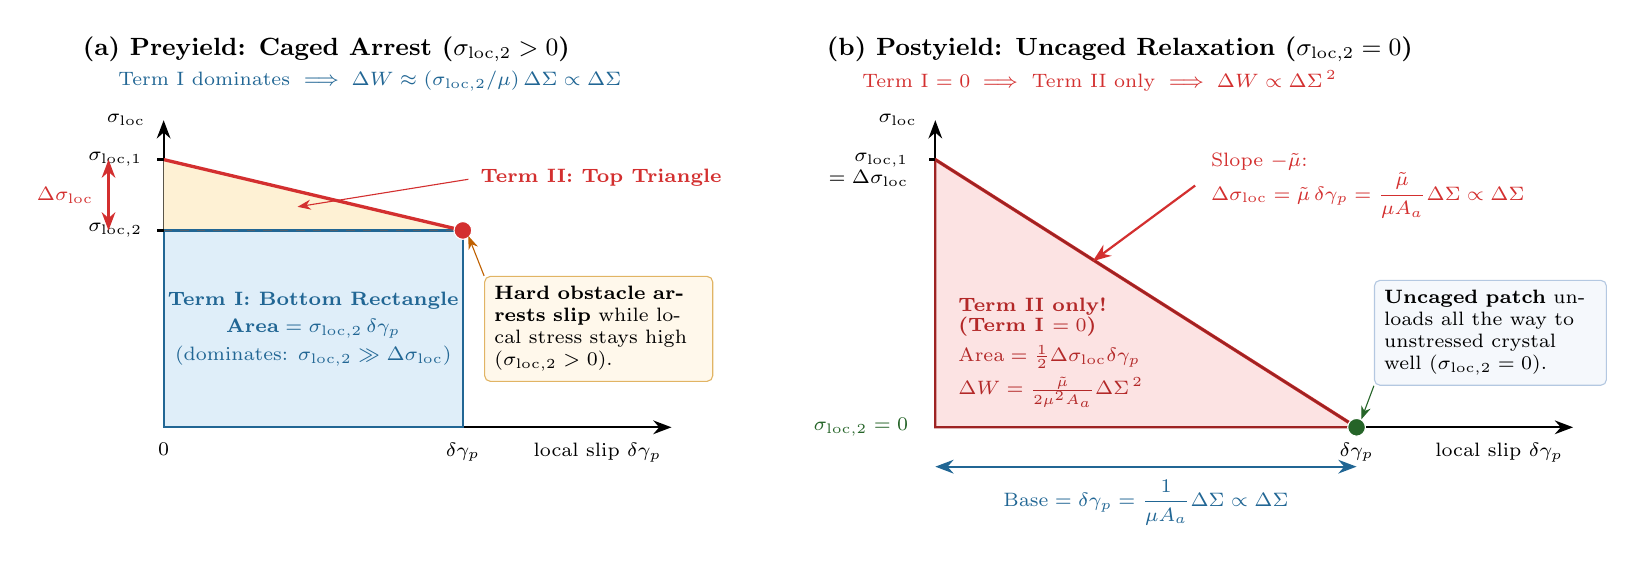
\begin{tikzpicture}[>=Stealth, font=\small]
  % ==================== PANEL (a): PREYIELD (x = 0..8.6) ====================
  \node[anchor=west, font=\bfseries\small] at (0.0, 5.55) {(a) Preyield: Caged Arrest ($\sigma_{\mathrm{loc},2} > 0$)};
  \node[anchor=west, font=\scriptsize, text=atomblue!80!black] at (0.45, 5.15) {Term I dominates $\implies \dW \approx (\sigma_{\mathrm{loc},2}/\mu)\,\dS \propto \dS$};

  % Axes
  \draw[->, thick] (1.15, 0.75) -- (7.60, 0.75) node[below=2pt, anchor=north east, font=\scriptsize] {local slip $\dgamp$};
  \draw[->, thick] (1.15, 0.75) -- (1.15, 4.65) node[left=3pt, font=\scriptsize] {$\sigloc$};

  % Coordinates: base from x=1.15 to x=4.95 (width = 3.80)
  % sigma_2 = y = 3.25, sigma_1 = y = 4.15
  \fill[softblue!90] (1.15, 0.75) rectangle (4.95, 3.25);
  \fill[softamber!95] (1.15, 3.25) -- (4.95, 3.25) -- (1.15, 4.15) -- cycle;

  % Outlines and unloading line
  \draw[thick, atomblue!80!black] (1.15, 0.75) rectangle (4.95, 3.25);
  \draw[very thick, defectred] (1.15, 4.15) -- (4.95, 3.25);
  \draw[dashed, slateh] (1.15, 3.25) -- (4.95, 3.25);

  % Y-axis ticks & labels
  \draw[thick] (1.07, 3.25) -- (1.15, 3.25) node[left=4pt, font=\scriptsize] {$\sigma_{\mathrm{loc},2}$};
  \draw[thick] (1.07, 4.15) -- (1.15, 4.15) node[left=4pt, font=\scriptsize] {$\sigma_{\mathrm{loc},1}$};
  \node[below=2pt, font=\scriptsize] at (1.15, 0.75) {$0$};
  \node[below=2pt, font=\scriptsize] at (4.95, 0.75) {$\dgamp$};

  % Labels cleanly inside blue rectangle (width ~3.2cm < 3.8cm)
  \node[font=\scriptsize\bfseries, text=atomblue!80!black, align=center] at (3.05, 2.00)
    {Term I: Bottom Rectangle\\[2pt] $\text{Area} = \sigma_{\mathrm{loc},2}\,\dgamp$\\[2pt] {\mdseries(dominates: $\sigma_{\mathrm{loc},2} \gg \dsigloc$)}};
  \node[font=\scriptsize\bfseries, text=defectred, anchor=west] at (5.05, 3.92) {Term II: Top Triangle};
  \draw[->, thin, defectred] (5.02, 3.90) -- (2.85, 3.55);

  % Dimension bracket for Delta sigma_loc
  \draw[<->, thick, defectred] (0.45, 3.25) -- (0.45, 4.15);
  \node[font=\scriptsize, text=defectred, left=2pt] at (0.45, 3.70) {$\dsigloc$};

  % Arrest annotation cleanly in right open area
  \filldraw[fill=defectred, draw=white] (4.95, 3.25) circle (3.2pt);
  \node[draw=warnframe, fill=warnbg, rounded corners=2pt, inner sep=3.5pt, font=\scriptsize, anchor=west, text width=2.65cm] (obs) at (5.22, 2.00)
    {\textbf{Hard obstacle arrests slip} while local stress stays high ($\sigma_{\mathrm{loc},2}>0$).};
  \draw[->, thin, orange!75!black] (obs.north west) -- (5.02, 3.18);

  % ==================== PANEL (b): POSTYIELD (x = 9.4..19.5) ====================
  \node[anchor=west, font=\bfseries\small] at (9.45, 5.55) {(b) Postyield: Uncaged Relaxation ($\sigma_{\mathrm{loc},2} = 0$)};
  \node[anchor=west, font=\scriptsize, text=defectred] at (9.90, 5.15) {Term I $= 0 \implies$ Term II only $\implies \dW \propto \dS^{\,2}$};

  % Axes
  \draw[->, thick] (10.95, 0.75) -- (19.05, 0.75) node[below=2pt, anchor=north east, font=\scriptsize] {local slip $\dgamp$};
  \draw[->, thick] (10.95, 0.75) -- (10.95, 4.65) node[left=3pt, font=\scriptsize] {$\sigloc$};

  % Triangle base x = 10.95 to 16.30 (width 5.35), height sigma_1 = y = 4.15
  \fill[softred!95] (10.95, 0.75) -- (16.30, 0.75) -- (10.95, 4.15) -- cycle;
  \draw[very thick, defectred] (10.95, 4.15) -- (16.30, 0.75);
  \draw[thick, defectred!75!black] (10.95, 0.75) -- (16.30, 0.75) -- (10.95, 4.15) -- cycle;

  % Height labels
  \draw[thick] (10.87, 4.15) -- (10.95, 4.15);
  \node[left=4pt, font=\scriptsize, align=right] at (10.87, 4.02) {$\sigma_{\mathrm{loc},1}$\\$=\dsigloc$};
  \node[left=4pt, font=\scriptsize, text=okgreen!80!black] at (10.87, 0.75) {$\sigma_{\mathrm{loc},2}=0$};

  % Base & Height callouts
  \draw[<->, thick, atomblue!80!black] (10.95, 0.25) -- (16.30, 0.25)
    node[midway, below=1pt, font=\scriptsize, text=atomblue!80!black] {$\text{Base} = \dgamp = \dfrac{1}{\mu A_a}\dS \propto \dS$};
  \node[below=2pt, font=\scriptsize] at (16.30, 0.75) {$\dgamp$};

  \draw[<-, thick, defectred] (12.95, 2.86) -- (14.25, 3.82)
    node[right=2pt, font=\scriptsize, align=left, text=defectred] {Slope $-\mutil$:\\ $\dsigloc = \mutil\,\dgamp = \dfrac{\mutil}{\mu A_a}\dS \propto \dS$};

  % Inside triangle text aligned cleanly inside lower-left corner
  \node[font=\scriptsize, text=defectred!85!black, align=left, anchor=south west] at (11.12, 0.88)
    {\textbf{Term II only!}\\[-1pt]
     \textbf{(Term I $= 0$)}\\[3pt]
     $\text{Area} = \tfrac{1}{2}\dsigloc\dgamp$\\[2pt]
     $\dW = \tfrac{\mutil}{2\mu^2 A_a}\dS^{\,2}$};

  % Endpoint dot + callout completely outside to the right
  \filldraw[fill=okgreen!80!black, draw=white] (16.30, 0.75) circle (3.2pt);
  \node[draw=boxframe, fill=boxbg, rounded corners=2pt, inner sep=3.5pt, font=\scriptsize, anchor=west, text width=2.70cm] (unc) at (16.52, 1.95)
    {\textbf{Uncaged patch} unloads all the way to unstressed crystal well ($\sigma_{\mathrm{loc},2}=0$).};
  \draw[->, thin, okgreen!80!black] (unc.south west) -- (16.36, 0.85);
\end{tikzpicture}%
}
\caption{\textbf{Trapezoid geometry explaining why Preyield is linear ($\gamma=1$) and Postyield is quadratic ($\gamma=2$).} \textbf{(a)}~In the caged preyield regime, hard obstacles arrest slip while $\sigma_{\mathrm{loc},2} > 0$, so the bottom rectangle (Term~I) dominates. \textbf{(b)}~In the uncaged postyield regime, no obstacle arrests the patch before its local driving stress relaxes to the unstressed square well ($\sigma_{\mathrm{loc},2}=0$); Term~I vanishes identically, leaving only the top triangle (Term~II).}
\label{fig:trapezoid}
\end{figure}

Comparing the two physical regimes in Figure~\ref{fig:trapezoid}:
\begin{itemize}[nosep]
  \item \textbf{Preyield (State~A, caged microplasticity):} Isolated 0D clusters ($D_\epsilon \approx 0.36$) slip inside a positively stressed matrix until arrested abruptly by pre-existing dislocation locks while $\sigma_{\mathrm{loc},2}$ is still high ($\sigma_{\mathrm{loc},2} \gg \dsigloc$). Thus the tall \textbf{Bottom Rectangle (Term I)} dominates, giving $\dW \approx \sigma_{\mathrm{loc},2} A_a \dgamp = (\sigma_{\mathrm{loc},2}/\mu)\,\dS \propto \dS$ ($\gamma=1$).
  \item \textbf{Postyield (State~D, marginally stable steady state):} As explained on p.~11 of PRM 2026, avalanches are no longer caged by regular arrays of hard obstacles. The active zone relaxes freely along the $\mathrm{GL}(2,\Z)$ valleys into the unstressed square-lattice grain interior ($\sigma_{\mathrm{loc},2} \approx 0$, white patches in Fig.~7 of PRM 2026). The bottom rectangle disappears ($\text{Term I} = 0$), leaving \textbf{only Term II}.
\end{itemize}

\subsection{Step-by-Step Proof That \texorpdfstring{$\text{Term II} \propto \dS^{\,2}$}{Term II propto Delta Sigma\textasciicircum 2}}

Take a uniform active patch $\Omega_a$ of area $A_a$ unloading locally by $\dsigloc$ over plastic slip $\dgamp$. Integrating the top triangle area $\frac{1}{2}\dsigloc\,\dgamp$ over $\Omega_a$ gives:
\begin{equation}
\label{eq:term2_base}
\text{Term II} = A_a \cdot \frac{1}{2}\cdot \underbrace{\dsigloc}_{\text{Height}} \cdot \underbrace{\dgamp}_{\text{Base}}.
\end{equation}
Why is there a factor of $\frac{1}{2}$? When $\sigma_{\mathrm{loc},2} = 0$, the local stress driving slip does \emph{not} stay fixed at $\dsigloc$ throughout the avalanche --- it starts at $\sigma_{\mathrm{loc},1} = \dsigloc$ and drops linearly to $0$, so the average stress doing work is $\frac{1}{2}\dsigloc$ (exactly like unloading a linear spring from force $\Delta F$ to $0$).

Now express \textbf{both} the Base ($\dgamp$) and the Height ($\dsigloc$) in terms of the macroscopic observable $\dS \equiv A\,\dsigbar$:
\begin{enumerate}[label=\textbf{Step \Alph*:}, leftmargin=4.2em]
  \item \textbf{Base ($\dgamp$) in terms of $\dS$.} By~\eqref{eq:hard_device} and the box-averaged plastic strain definition in Table~\ref{tab:symbols}:
  \[
  \dS = A\,\dsigbar = A\left(\mu\,\Delta\bar{\gamma}_p\right) = A\left(\mu\,\frac{A_a}{A}\,\dgamp\right) = \mu\,A_a\,\dgamp
  \qquad\Longrightarrow\qquad
  \dgamp = \frac{1}{\mu\,A_a}\,\dS.
  \]
  (Notice how the box area $A$ cancels. Physically, at fixed active area $A_a$, an avalanche with $2\times$ larger $\dS$ slipped $2\times$ further: $\text{Base}\propto\dS$.)
  \item \textbf{Height ($\dsigloc$) in terms of $\dS$.} By local linear elasticity / Eshelby inclusion unloading inside $\Omega_a$, $\dsigloc = \mutil\,\dgamp$, where $\mutil \in (0,\mu]$ accounts for the elastic compliance of the surrounding matrix $\Omega_m$. Substituting Step~A:
  \[
  \dsigloc = \mutil\left(\frac{1}{\mu\,A_a}\,\dS\right) = \frac{\mutil}{\mu\,A_a}\,\dS.
  \]
  (Physically, because $\sigma_{\mathrm{loc},2}=0$, slipping $2\times$ further means the patch must have started from a $2\times$ higher local stress $\sigma_{\mathrm{loc},1} = \dsigloc$: $\text{Height}\propto\dS$.)
  \item \textbf{Multiply $A_a \times \frac{1}{2} \times \text{Height} \times \text{Base}$.} Substituting Steps~A and B into~\eqref{eq:term2_base}:
  \begin{equation}
  \label{eq:term2_final}
  \text{Term II} = A_a \cdot \frac{1}{2} \cdot \left(\frac{\mutil}{\mu\,A_a}\,\dS\right)\!\left(\frac{1}{\mu\,A_a}\,\dS\right)
  = \frac{\mutil}{2\,\mu^2\,A_a}\,(\dS)^2 \propto \dS^{\,2}.
  \end{equation}
\end{enumerate}

\noindent\textbf{Dimensional check:} $\dfrac{[\text{stress}]}{[\text{stress}]^2[\text{area}]}\,\big([\text{stress}][\text{area}]\big)^2 = [\text{stress}][\text{area}] = [\text{energy}]$. \checkmark

\begin{remark}[Extension to Nonlinear Elasticity (PRM 2026, p.~11)]
If the local constitutive unloading law is a power law $\dsigloc \propto (\dgamp)^\nu$, then $\text{Base} = \dgamp \propto (\dsigloc)^{1/\nu}$ and $\dsigloc \propto \dS$ (or at patch scale $\dW \sim \dsigloc\,\dgamp$), yielding $\dW \propto \dS^{\,\gamma}$ with $\gamma = 1 + 1/\nu$ (or $\gamma = 2$ for Hookean linear elasticity $\nu=1$, recovering p.~11 of PRM 2026: $\epsilon - 1 = (\tau - 1)/\gamma$ with $\gamma=2$).
\end{remark}

% ============================================================================
\section{Where Did \texorpdfstring{$(\sigbar/\mu)\dS$}{(sigma\_bar/mu) Delta Sigma} Go? Spatial Variance Cancellation \& Worked Example}
\label{sec:variance_cancellation}
% ============================================================================

How can Eq.~\eqref{eq:term2_final} give $\dW \propto \dS^{\,2}$ when Eq.~\eqref{eq:naive_homog} clearly shows $\Delta W_{\mathrm{macro}} \approx (\sigbar/\mu)\,\dS$? Decompose the shear stress field across the entire box into its spatial mean plus zero-mean fluctuations:
\[
\sigma_{xy}(\mathbf{x}) = \sigbar + \delta\sigma_{xy}(\mathbf{x}),
\qquad \int_{\Omega_0}\delta\sigma_{xy}(\mathbf{x})\,\mathrm{d}\mathbf{x} = 0.
\]
Because the cross term $2\sigbar\int_{\Omega_0}\delta\sigma_{xy}(\mathbf{x})\,\mathrm{d}\mathbf{x}$ vanishes \textbf{identically} by orthogonality, the total linear-elastic energy obeys an exact Pythagorean decomposition:
\begin{equation}
\label{eq:pythagoras}
W = \int_{\Omega_0}\frac{\big(\sigbar + \delta\sigma_{xy}(\mathbf{x})\big)^2}{2\mu}\,\mathrm{d}\mathbf{x}
= \underbrace{\frac{A}{2\mu}\,\sigbar^{\,2}}_{W_{\mathrm{macro}}}
\;+\; \underbrace{\int_{\Omega_0}\frac{\delta\sigma_{xy}(\mathbf{x})^2}{2\mu}\,\mathrm{d}\mathbf{x}}_{E_{\mathrm{inhom}}\text{ (stress variance)}},
\end{equation}
so every avalanche energy drop obeys:
\begin{equation}
\label{eq:exact_split_diff}
\dW = \Delta W_{\mathrm{macro}} - \Delta E_{\mathrm{inhom}},
\qquad
\Delta E_{\mathrm{inhom}} \equiv E_{\mathrm{inhom},2} - E_{\mathrm{inhom},1}.
\end{equation}
When a soft zone inside a stressed polycrystal relaxes to $\sigma_{a,2}=0$, it becomes \emph{more different} from the box mean $\sigbar > 0$ (whose internal stress fluctuations come from $\Sigma 5$ grain boundaries at $\pm 0.5$): its local fluctuation $|\delta\sigma_a| = |\sigma_a - \sigbar|$ widens from $|\sigma_{a,1}-\sigbar|$ to $\sigbar$, \textbf{storing $\Delta E_{\mathrm{inhom}} > 0$ into internal back-stress contrast} and almost completely cancelling $\Delta W_{\mathrm{macro}}$!

\begin{cautionbox}[Why $\nabla_{\mathbf{u}} W = \mathbf{0}$ Is \emph{Not} the Reason]
One should \emph{not} say ``the linear term vanishes because the final state minimizes energy ($\nabla_{\mathbf{u}} W(\mathbf{u}_2) = \mathbf{0}$).'' \textbf{Every} equilibrated MTM configuration --- both Preyield State~A and Postyield State~D --- satisfies $\nabla_{\mathbf{u}} W = \mathbf{0}$ (Eq.~29 of PRM 2026) with respect to displacements $\mathbf{u}$, \emph{at fixed integer lattice slips $\mathbf{m}$}. The difference between the two regimes is solely whether the local shear stress inside $\Omega_a$ arrests at a finite value ($\sigma_{\mathrm{loc},2} > 0 \implies$ linear) or unloads all the way to the unstressed crystal well ($\sigma_{\mathrm{loc},2} \approx 0 \implies$ quadratic).
\end{cautionbox}

\subsection{Worked Numerical Example (\texorpdfstring{$\sigbar = 0.13$, $\sigma_{a,1}=0.02 \to \sigma_{a,2}=0$}{sigma\_bar = 0.13, sigma\_a1 = 0.02 -> 0})}

Set $\mu = \mutil = 1$, active patch area $A_a = 1$ in a large crystal ($A \gg 1$) sitting on the postyield plateau at mean stress $\sigbar = 0.13$ (Figure~\ref{fig:variance_check}a). Suppose a partially shielded patch starts at $\sigma_{a,1} = 0.02$ and slips by $\dgamp = 0.02$ until $\sigma_{a,2} = 0$, giving extensive stress drop $\dS = \mu A_a \dgamp = 0.02$:
\begin{enumerate}[nosep]
  \item \textbf{Macroscopic elastic energy drop (Eq.~\ref{eq:naive_homog}, linear in $\dS$):}
  \[
  \Delta W_{\mathrm{macro}} \approx \frac{\sigbar}{\mu}\,\dS = 0.13 \times 0.02 = \mathbf{0.00260}.
  \]
  \item \textbf{Increase in inhomogeneous variance energy $E_{\mathrm{inhom}}$ (Eq.~\ref{eq:pythagoras}):}
  Inside $\Omega_a$, the deviation $\delta\sigma_a = \sigma_a - \sigbar$ deepens from $0.02 - 0.13 = -0.11$ to $0 - 0.13 = -0.13$ (Figure~\ref{fig:variance_check}a), while the outer matrix ($A\gg 1$) absorbs the tiny mean change $\Delta\sigbar = \dS/A$ with negligible $\mathcal{O}(1/A)$ variance contribution:
  \[
  \Delta E_{\mathrm{inhom}} = \frac{A_a}{2\mu}\Big[(-0.13)^2 - (-0.11)^2\Big]
  = \frac{1}{2}\big(0.0169 - 0.0121\big) = \mathbf{0.00240}.
  \]
  \item \textbf{Exact net dissipated energy $\dW = \Delta W_{\mathrm{macro}} - \Delta E_{\mathrm{inhom}}$:}
  \[
  \dW = 0.00260 - 0.00240 = \mathbf{0.00020} = \frac{1}{2}(0.02)^2 = \frac{1}{2}\,\dS^{\,2}.
  \]
\end{enumerate}
\textbf{General algebraic identity:} For \emph{any} plateau mean $\sigbar$ and \emph{any} local drop $\dsigloc \equiv \Delta\sigma$ relaxing to $\sigma_{a,2}=0$, the first-order $\sigbar\,\Delta\sigma$ terms cancel identically:
\begin{equation}
\label{eq:exact_identity}
\sigbar\,\Delta\sigma \;-\; \frac{1}{2}\Big[(-\sigbar)^2 - (\Delta\sigma - \sigbar)^2\Big]
= \sigbar\,\Delta\sigma \;-\; \Big[\sigbar\,\Delta\sigma - \frac{1}{2}\Delta\sigma^2\Big]
\;\equiv\; \frac{1}{2}\,\Delta\sigma^2.
\end{equation}
Including elastic compliance of the surrounding matrix ($0 < \mutil < \mu$) redistributes part of $\Delta E_{\mathrm{inhom}}$ into the matrix and replaces the prefactor $\frac{1}{2}$ by $\frac{\mutil}{2\mu^2 A_a}$, preserving the exact cancellation of the linear term.

\begin{figure}[ht!]
\centering
\resizebox{\textwidth}{!}{%
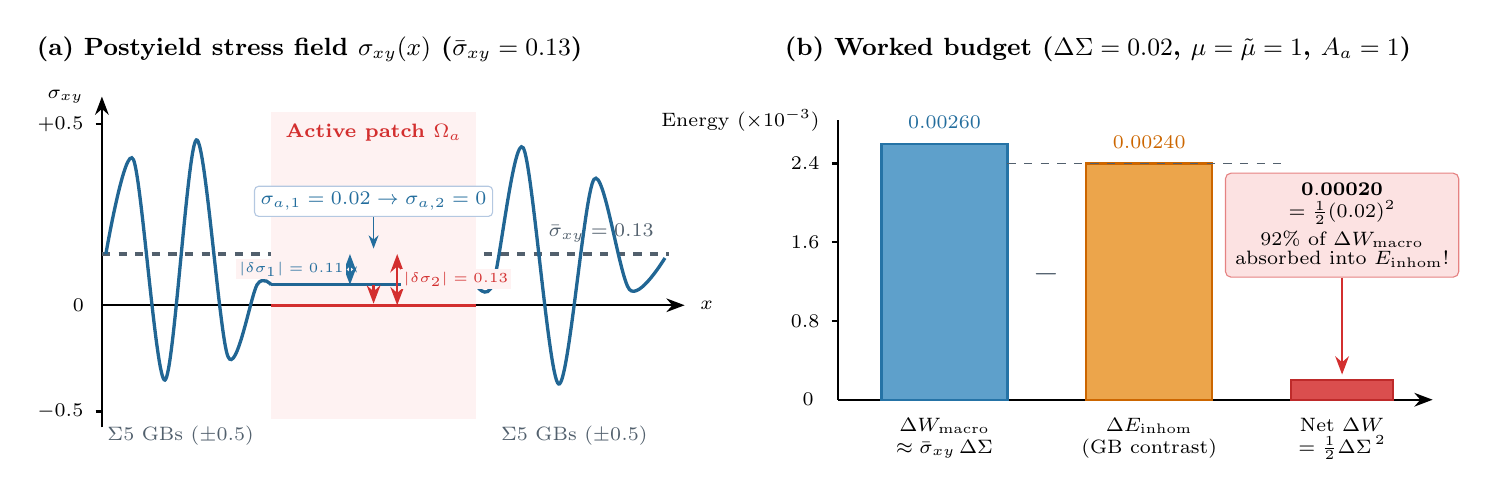
\begin{tikzpicture}[>=Stealth, font=\small]
  % ==================== PANEL (a): Spatial profile & contrast (x = 0..8.8) ====================
  \node[anchor=west, font=\bfseries\small] at (0.0, 5.25) {(a) Postyield stress field $\sigma_{xy}(x)$ ($\bar{\sigma}_{xy}=0.13$)};

  % Axes
  \draw[->, thick] (0.95, 2.00) -- (8.35, 2.00) node[right=2pt, font=\scriptsize] {$x$};
  \draw[->, thick] (0.95, 0.45) -- (0.95, 4.65) node[left=3pt, font=\scriptsize] {$\sigma_{xy}$};
  \node[left=3pt, font=\scriptsize] at (0.95, 2.00) {$0$};
  \draw[thick] (0.87, 4.30) -- (0.95, 4.30) node[left=3pt, font=\scriptsize] {$+0.5$};
  \draw[thick] (0.87, 0.65) -- (0.95, 0.65) node[left=3pt, font=\scriptsize] {$-0.5$};

  % Mean plateau line sigma_bar = 0.13 -> y = 2.65
  \draw[dashed, slateh, very thick] (0.95, 2.65) -- (8.15, 2.65);
  \node[font=\scriptsize, text=slateh, anchor=south west] at (6.50, 2.68) {$\sigbar = 0.13$};

  % Shaded active patch Omega_a: x from 3.10 to 5.70 (width 2.60 cm)
  \fill[softred!45] (3.10, 0.55) rectangle (5.70, 4.45);
  \node[font=\scriptsize\bfseries, text=defectred, anchor=north] at (4.40, 4.42) {Active patch $\Omega_a$};

  % Stress profile: GB spikes on left & right, flat plateau at sigma_{a,1}=0.02 across Omega_a
  \draw[very thick, atomblue!80!black, smooth]
    plot coordinates {(1.00, 2.65) (1.35, 3.85) (1.75, 1.05) (2.15, 4.10) (2.55, 1.35) (2.92, 2.26) (3.10, 2.26)};
  \draw[very thick, atomblue!80!black] (3.10, 2.26) -- (5.70, 2.26);
  \draw[very thick, atomblue!80!black, smooth]
    plot coordinates {(5.70, 2.26) (5.92, 2.28) (6.30, 4.00) (6.75, 1.00) (7.20, 3.60) (7.65, 2.20) (8.10, 2.60)};
  % State 2 inside Omega_a drops to sigma_{a,2}=0 (y=2.00)
  \draw[very thick, defectred] (3.10, 2.00) -- (5.70, 2.00);
  \draw[->, thick, defectred] (4.40, 2.26) -- (4.40, 2.02);

  % Annotations for delta sigma_a widening cleanly inside Omega_a
  \draw[<->, thick, atomblue!85!black] (4.10, 2.26) -- (4.10, 2.65);
  \node[font=\tiny, text=atomblue!85!black, fill=softred!45, inner sep=1pt, anchor=east] at (4.06, 2.46) {$|\delta\sigma_1|=0.11$};
  \draw[<->, thick, defectred] (4.70, 2.00) -- (4.70, 2.65);
  \node[font=\tiny, text=defectred, fill=softred!45, inner sep=1pt, anchor=west] at (4.74, 2.33) {$|\delta\sigma_2|=0.13$};

  \node[font=\scriptsize, text=slateh, align=center] at (1.95, 0.35) {$\Sigma 5$ GBs ($\pm 0.5$)};
  \node[font=\scriptsize, text=slateh, align=center] at (6.95, 0.35) {$\Sigma 5$ GBs ($\pm 0.5$)};
  \node[draw=boxframe, fill=white, rounded corners=1.5pt, inner sep=2.2pt, font=\scriptsize, text=atomblue!85!black] (stnote) at (4.40, 3.32)
    {$\sigma_{a,1}=0.02 \to \sigma_{a,2}=0$};
  \draw[->, thin, atomblue!85!black] (stnote.south) -- (4.40, 2.72);

  % ==================== PANEL (b): Numerical Energy Budget (x = 9.5..18.6) ====================
  \node[anchor=west, font=\bfseries\small] at (9.50, 5.25) {(b) Worked budget ($\dS = 0.02$, $\mu=\mutil=1$, $A_a=1$)};

  % Baseline at y=0.80, scale 0.0026 -> height 3.25 cm (0.0001 -> 0.125 cm)
  \draw[->, thick] (10.30, 0.80) -- (17.85, 0.80);
  \draw[thick] (10.30, 0.80) -- (10.30, 4.35) node[left=3pt, font=\scriptsize] {Energy ($\times 10^{-3}$)};
  \foreach \ylab in {0.8, 1.6, 2.4} {
    \draw[thick] (10.22, {0.80 + \ylab*1.25}) -- (10.30, {0.80 + \ylab*1.25}) node[left=3pt, font=\scriptsize] {$\ylab$};
  }
  \node[left=3pt, font=\scriptsize] at (10.22, 0.80) {$0$};

  % Bar 1: Delta W_macro = 0.00260 -> height = 2.60 * 1.25 = 3.25
  \fill[atomblue!75] (10.85, 0.80) rectangle (12.45, 4.05);
  \draw[thick, atomblue!90!black] (10.85, 0.80) rectangle (12.45, 4.05);
  \node[font=\scriptsize\bfseries, above=2pt, text=atomblue!85!black] at (11.65, 4.05) {$0.00260$};
  \node[font=\scriptsize, align=center, below=3pt] at (11.65, 0.80) {$\Delta W_{\mathrm{macro}}$\\$\approx\sigbar\,\dS$};

  % Minus sign
  \node[font=\large\bfseries, text=slateh] at (12.95, 2.40) {$-$};

  % Bar 2: Delta E_inhom = 0.00240 -> height = 2.40 * 1.25 = 3.00
  \fill[amberh!75] (13.45, 0.80) rectangle (15.05, 3.80);
  \draw[thick, orange!80!black] (13.45, 0.80) rectangle (15.05, 3.80);
  \node[font=\scriptsize\bfseries, above=2pt, text=orange!80!black] at (14.25, 3.80) {$0.00240$};
  \node[font=\scriptsize, align=center, below=3pt] at (14.25, 0.80) {$\Delta E_{\mathrm{inhom}}$\\(GB contrast)};

  % Equals sign
  \node[font=\large\bfseries, text=slateh] at (15.55, 2.40) {$=$};

  % Bar 3: Net Delta W = 0.00020 -> height = 0.20 * 1.25 = 0.25
  \fill[defectred!85] (16.05, 0.80) rectangle (17.35, 1.05);
  \draw[thick, defectred!90!black] (16.05, 0.80) rectangle (17.35, 1.05);
  \node[font=\scriptsize, align=center, below=3pt] at (16.70, 0.80) {Net $\dW$\\$=\frac{1}{2}\dS^{\,2}$};

  % Callout for tiny remainder bar
  \node[draw=defectred!60, fill=softred, rounded corners=2pt, inner sep=3.5pt, font=\scriptsize, align=center, anchor=south] (netbox) at (16.70, 2.35)
    {$\mathbf{0.00020}$\\$=\frac{1}{2}(0.02)^2$\\[2pt]\scriptsize $92\%$ of $\Delta W_{\mathrm{macro}}$\\[-1pt]\scriptsize absorbed into $E_{\mathrm{inhom}}$!};
  \draw[->, thick, defectred] (netbox.south) -- (16.70, 1.12);

  % Guide line across bars
  \draw[dashed, slateh] (12.45, 3.80) -- (15.95, 3.80);
\end{tikzpicture}%
}
\caption{\textbf{Why the linear $\sigbar\,\dS$ term cancels on the postyield plateau.} \textbf{(a)}~When an active patch unloads from $\sigma_{a,1}=0.02$ to $\sigma_{a,2}=0$ inside a polycrystal of mean $\sigbar=0.13$, its deviation $|\delta\sigma_a|=|\sigma_a-\sigbar|$ widens from $0.11$ to $0.13$, storing $\Delta E_{\mathrm{inhom}}$ in internal stress contrast against the $\Sigma 5$ grain boundaries. \textbf{(b)}~For the worked numbers, $92\%$ of $\Delta W_{\mathrm{macro}}$ cancels out, leaving $\dW = \frac{1}{2}\dS^{\,2} = 0.00020$.}
\label{fig:variance_check}
\end{figure}

% ============================================================================
\section{Global Plateau Conservation, Fractal Dimensions (\texorpdfstring{$D_\epsilon, D_\tau$}{D\_eps, D\_tau}), and Synthesis}
\label{sec:global_balance}
% ============================================================================

\subsection{Reconciling Individual Quadratic Drops (\texorpdfstring{$\gamma=2$}{gamma=2}) with Global Linearity (\texorpdfstring{$\langle\dW\rangle \propto \langle\dS\rangle$}{<Delta W> propto <Delta Sigma>})}

A subtle consistency check arises on the stationary postyield plateau ($\mathrm{d}\langle W\rangle/\mathrm{d}\alpha = 0$ on average): globally, external boundary work over a long strain interval $\Delta\alpha$ must balance total dissipated avalanche energy:
\begin{equation}
\sum_{k} \Delta W_k = A\,\sigbar\,\Delta\alpha_{\mathrm{tot}}
= A\,\sigbar\left(\Delta\bar{\gamma}_e^{\mathrm{rem}} + \frac{\sum_k \Delta\Sigma_k}{\mu A}\right)
\qquad\Longrightarrow\qquad
\frac{\langle \dW \rangle}{\langle \dS \rangle} \approx \frac{\sigbar}{\mu_{\mathrm{eff}}} = \mathcal{O}(1),
\end{equation}
independent of box size $L$! How can the \emph{ensemble ratio} $\langle \dW \rangle / \langle \dS \rangle$ stay $\mathcal{O}(1)$ as $L\to\infty$ if \emph{individual} events follow $\dW \sim \dS^{\,2}/A_a$?

The answer lies in the \textbf{different finite-size cutoffs} $L^{D_\epsilon}$ and $L^{D_\tau}$ measured in Fig.~10 of PRM 2026:
\begin{enumerate}[nosep]
  \item Integrating the first moment of $P(s;L) = s^{-x}\mathcal{F}(s/L^{D_x})$ for $1 < x < 2$ (or near $x\approx 1$) gives $\langle s \rangle \sim L^{D_x(2-x)}$. Plugging in the \textbf{Postyield exponents} from Table~\ref{tab:prm_exponents}:
  \begin{equation}
  D_\epsilon(2-\epsilon) = 0.9836\,(2 - 1.0207) = \mathbf{0.963} \approx 1,
  \qquad
  D_\tau(2-\tau) = 1.4379\,(2 - 1.2476) = \mathbf{1.082} \approx 1.
  \end{equation}
  Both mean dissipated energy $\langle\dW\rangle \sim L^1$ and mean extensive stress drop $\langle\dS\rangle \sim L^1$ scale with the exact same system-size exponent $L^1$, keeping $\langle\dW\rangle/\langle\dS\rangle = \mathcal{O}(1)$ globally!
  \item Geometrically, for a spanning 1D-like branched avalanche (Fig.~11 of PRM 2026) whose active length $\ell \sim L$, Eq.~\eqref{eq:term2_final} gives $\dW_{\max} \sim \dS_{\max}^2 / (\mu\,L^2)$ at cutoff scale, predicting $D_\epsilon \approx 2 D_\tau - 2 = 2(1.4379) - 2 = \mathbf{0.88}$ (close to the measured $D_\epsilon = 0.98 \pm 0.1$, because the local unloading stiffness of a spanning shear band scales more weakly than $1/L^2$).
\end{enumerate}

\begin{figure}[ht!]
\centering
\resizebox{\textwidth}{!}{%
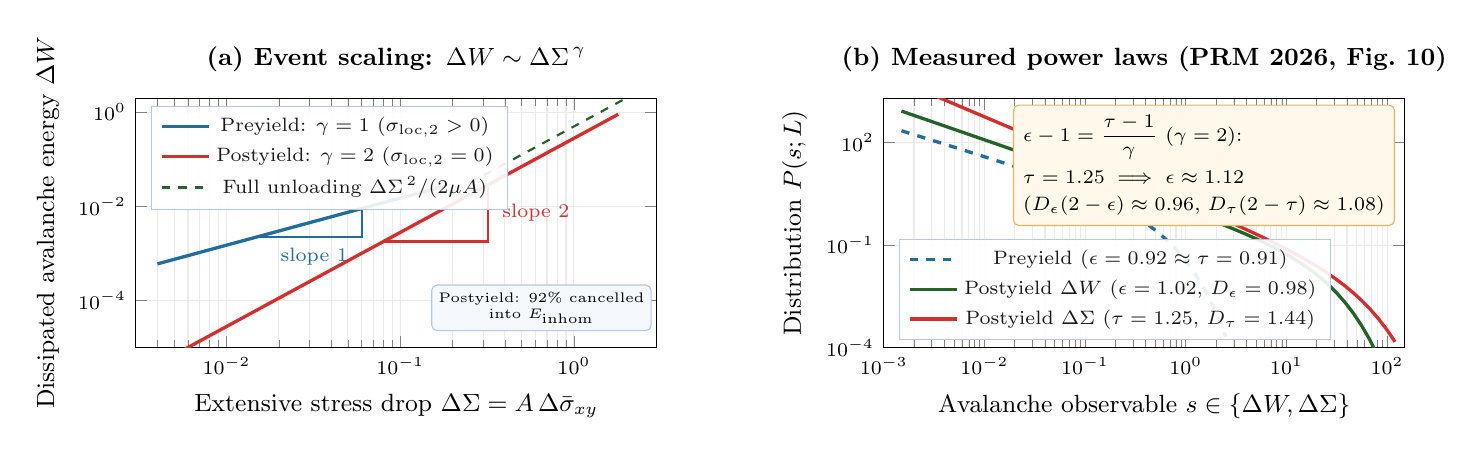
\begin{tikzpicture}[font=\small]
  % ==================== PANEL (a): Delta W vs Delta Sigma ====================
  \begin{axis}[
    name=ax1,
    at={(0,0)},
    width=8.2cm, height=4.75cm,
    xmode=log, ymode=log,
    xmin=3e-3, xmax=3e0,
    ymin=1e-5, ymax=2e0,
    xlabel={Extensive stress drop $\dS = A\,\dsigbar$},
    ylabel={Dissipated avalanche energy $\dW$},
    title={\textbf{(a) Event scaling: $\dW \sim \dS^{\,\gamma}$}},
    title style={font=\small},
    label style={font=\small},
    tick label style={font=\scriptsize},
    grid=both,
    grid style={black!8},
    legend pos=north west,
    legend style={font=\scriptsize, fill=white, fill opacity=0.9, draw=boxframe},
  ]
    % Preyield gamma = 1: y = 0.15 * x
    \addplot[atomblue!85!black, very thick, domain=4e-3:1.8e-1] {0.15*x};
    \addlegendentry{Preyield: $\gamma=1$ ($\sigma_{\mathrm{loc},2}>0$)}

    % Postyield gamma = 2: y = 0.28 * x^2 (Eshelby effective compliance tilde_mu < mu)
    \addplot[defectred, very thick, domain=4e-3:1.8e0] {0.28*x^2};
    \addlegendentry{Postyield: $\gamma=2$ ($\sigma_{\mathrm{loc},2}=0$)}

    % Asymptotic full unloading line (uniform box: y = 0.5 * x^2)
    \addplot[okgreen!80!black, dashed, thick, domain=2.5e-1:2.2e0] {0.5*x^2};
    \addlegendentry{Full unloading $\dS^{\,2}/(2\mu A)$}

    % Slope triangles
    \draw[atomblue!85!black, thick] (axis cs:0.015,0.00225) -- (axis cs:0.06,0.00225) -- (axis cs:0.06,0.009);
    \node[text=atomblue!85!black, font=\scriptsize, anchor=north] at (axis cs:0.032,0.0021) {slope $1$};

    \draw[defectred, thick] (axis cs:0.08,0.001792) -- (axis cs:0.32,0.001792) -- (axis cs:0.32,0.028672);
    \node[text=defectred, font=\scriptsize, anchor=west] at (axis cs:0.34,0.0075) {slope $2$};

    % Crossover note
    \node[draw=boxframe, fill=boxbg, rounded corners=2pt, inner sep=2.5pt, font=\tiny, align=center]
      at (axis cs:0.65,7.0e-5) {Postyield: $92\%$ cancelled\\into $E_{\mathrm{inhom}}$};
  \end{axis}

  % ==================== PANEL (b): PDF exponents & cutoff scaling ====================
  \begin{axis}[
    name=ax2,
    at={(9.5cm,0)},
    width=8.2cm, height=4.75cm,
    xmode=log, ymode=log,
    xmin=1e-3, xmax=1.5e2,
    ymin=1e-4, ymax=2e3,
    xlabel={Avalanche observable $s \in \{\dW, \dS\}$},
    ylabel={Distribution $P(s; L)$},
    title={\textbf{(b) Measured power laws (PRM 2026, Fig.~10)}},
    title style={font=\small},
    label style={font=\small},
    tick label style={font=\scriptsize},
    grid=both,
    grid style={black!8},
    legend pos=south west,
    legend style={font=\scriptsize, fill=white, fill opacity=0.9, draw=boxframe},
  ]
    % Preyield P(s) ~ s^-0.91 exp(-s/0.5)
    \addplot[atomblue!85!black, very thick, dashed, domain=1.5e-3:2.5e0, samples=60] {0.6*(x^-0.91)*exp(-x/0.35)};
    \addlegendentry{Preyield ($\epsilon=0.92 \approx \tau=0.91$)}

    % Postyield P(Delta W) ~ x^-1.02 exp(-x/15)
    \addplot[okgreen!80!black, very thick, domain=1.5e-3:8e1, samples=60] {1.1*(x^-1.02)*exp(-x/15.0)};
    \addlegendentry{Postyield $\dW$ ($\epsilon=1.02$, $D_\epsilon=0.98$)}

    % Postyield P(Delta Sigma) ~ x^-1.25 exp(-x/40)
    \addplot[defectred, very thick, domain=1.5e-3:1.2e2, samples=60] {1.8*(x^-1.25)*exp(-x/35.0)};
    \addlegendentry{Postyield $\dS$ ($\tau=1.25$, $D_\tau=1.44$)}

    % Annotation box connecting them
    \node[draw=warnframe, fill=warnbg, rounded corners=2pt, inner sep=3.5pt, font=\scriptsize, align=left, anchor=north east]
      at (axis cs:120,1300) {
        $\epsilon - 1 = \dfrac{\tau - 1}{\gamma}$ ($\gamma=2$):\\[3pt]
        $\tau=1.25 \implies \epsilon \approx 1.12$\\[2pt]
        \scriptsize ($D_\epsilon(2-\epsilon)\approx 0.96$, $D_\tau(2-\tau)\approx 1.08$)
      };
  \end{axis}
\end{tikzpicture}%
}
\caption{\textbf{Summary of event-level and ensemble-level avalanche scaling in MTM.} \textbf{(a)}~Preyield caged events obey linear scaling ($\gamma=1$) because $\sigma_{\mathrm{loc},2}>0$, whereas uncaged postyield events drop to $\sigma_{\mathrm{loc},2}=0$ and follow $\gamma=2$. \textbf{(b)}~Resulting power-law distributions matching \emph{Phys.\ Rev.\ Mater.}\ \textbf{10}, 103611 (2026), Fig.~10.}
\label{fig:scaling_plots}
\end{figure}

\subsection{Master Regime Comparison Table}

Table~\ref{tab:master_summary} compares all three unloading regimes across AQS and hydrogen-coupled MTM.

\begin{table}[ht!]
\centering
\caption{\textbf{Side-by-side synthesis of all MTM avalanche unloading regimes.}}
\label{tab:master_summary}
\footnotesize
\setlength{\tabcolsep}{4.5pt}
\begin{tabular}{@{}L{2.7cm}L{2.75cm}L{2.8cm}L{2.9cm}L{3.45cm}@{}}
\toprule
\textbf{Regime} & \textbf{Arrest mechanism} & \textbf{Local final stress $\sigma_{\mathrm{loc},2}$} & \textbf{Energy vs.\ $\dS$} & \textbf{Physical signature} \\
\midrule
\textbf{Preyield} (State A) &
Dislocation locks arrest small 0D clusters ($D_\epsilon \approx 0.36$) &
$\sigma_{\mathrm{loc},2} > 0$ (Term~I rectangle dominates) &
\textbf{Linear ($\gamma=1$):}\newline $\dW \approx \frac{\sigma_{\mathrm{loc},2}}{\mu}\dS$ &
$\tau\approx\epsilon\approx 0.91$; strong hardening; caged slip \\[2.5pt]
\textbf{Postyield plateau} (State D) &
Uncaged 1D bands ($D_\epsilon \approx 0.98$) relax into unstressed grain wells &
$\sigma_{\mathrm{loc},2} \approx 0$ (Term~I $=0$, Term~II triangle only) &
\textbf{Quadratic ($\gamma=2$):}\newline $\dW \approx \frac{\mutil}{2\mu^2 A_a}\dS^{\,2}$ &
$\tau\approx 1.25$, $\epsilon\approx 1.02$; $92\%$ of $\Delta W_{\mathrm{macro}}$ absorbed into $E_{\mathrm{inhom}}$ \\[2.5pt]
\textbf{Pristine spinodal / H breakaway} &
Global cascade at $\alpha_c\approx 0.138$, or unpinning above $\tau_P^0+\Delta\tau_{\mathrm{age}}(t_w)$ &
$\bar{\sigma}_{xy,2}\to 0$ (full unload) or $\tau_P^0$ (partial H-PLC drop) &
Full: $\frac{\dS^2}{2\mu A}$;\newline H-PLC: $\frac{A\bar{\tau}}{\mu}\dsigbar - \Delta E_{\mathrm{H\text{-}bind}}$ &
$N_{\mathrm{sweeps}} = \frac{\bar{\sigma}_{xy,1}}{\mu}\frac{L_y}{b}$, or $n_{\mathrm{jump}}\sim \frac{\Delta\tau_{\mathrm{age}}}{\mu}\big(\frac{L}{b}\big)^2$ hops \\
\bottomrule
\end{tabular}
\end{table}

% ============================================================================
\vspace{-6pt}
\begin{thebibliography}{9}
\small
\setlength{\itemsep}{1pt}
\setlength{\parsep}{0pt}
\bibitem{Salman2026PRM}
O.~U.\ Salman, A.~Ahadi, and L.~Truskinovsky,
\emph{Self-induced marginality in plastically deformed crystals},
Phys.\ Rev.\ Mater.\ \textbf{10}, 103611 (2026).
\url{https://doi.org/10.1103/3rwf-d3yx}

\bibitem{ContiZanzotto2004}
S.~Conti and G.~Zanzotto,
\emph{A variational model for reconstructive phase transformations in crystals, and their relation to dislocations and plasticity},
Arch.\ Ration.\ Mech.\ Anal.\ \textbf{173}, 69--88 (2004).

\bibitem{Shang2020PNAS}
B.~Shang, P.~Guan, and J.-L.\ Barrat,
\emph{Elastic avalanches reveal marginal behavior in amorphous solids},
Proc.\ Natl.\ Acad.\ Sci.\ U.S.A.\ \textbf{117}, 86--92 (2020).

\bibitem{Lin2014PNAS}
J.~Lin, E.~Lerner, A.~Rosso, and M.~Wyart,
\emph{Scaling description of the yielding transition in soft amorphous solids at zero temperature},
Proc.\ Natl.\ Acad.\ Sci.\ U.S.A.\ \textbf{111}, 14382--14387 (2014).

\bibitem{Ispanovity2014PRL}
P.~D.\ Isp\'anovity, L.~Laurson, M.~Zaiser, I.~Groma, S.~Zapperi, and M.~J.\ Alava,
\emph{Avalanches in 2D dislocation systems: Plastic yielding is not depinning},
Phys.\ Rev.\ Lett.\ \textbf{112}, 235501 (2014).
\end{thebibliography}

\end{document}
